\documentclass{article}
\usepackage{neurips_2019}

\usepackage[utf8]{inputenc} % allow utf-8 input
\usepackage[T1]{fontenc}    % use 8-bit T1 fonts
\usepackage[usenames, svgnames]{xcolor}
\usepackage{hyperref}       % hyperlinks
\usepackage{bchart}
\usepackage{pgfplots}
\pgfplotsset{width=7 cm,compat=1.5}
\hypersetup{
	colorlinks=true,
	linkcolor={red!80!black},
	%	citecolor={blue!80!black},
	%	urlcolor={magenta}
}

\usepackage{url}            % simple URL typesetting
\usepackage{booktabs}       % professional-quality tables
\usepackage{amsfonts}       % blackboard math symbols
\usepackage{nicefrac}       % compact symbols for 1/2, etc.
\usepackage{microtype}      % microtypography
\usepackage{graphicx}

% Useful packages
\usepackage{amsmath, amssymb, amsfonts, bm}
\usepackage{amsthm}
\usepackage{mathtools}
%\usepackage[usenames, dvipsnames]{color}
\usepackage{cleveref}
\crefname{figure}{Figure}{Figures}

%\usepackage{enumitem}
%\setlist[enumerate]{labelindent=5pt, label=\alph*)} 


% \usepackage{blindtext}

\newtheorem{theorem}{Theorem}
\newtheorem{proposition}[theorem]{Proposition}
\newtheorem{corollary}[theorem]{Corollary}
\newtheorem{lemma}[theorem]{Lemma}
\newtheorem{remark}[theorem]{Remark}

\theoremstyle{remark}
\newtheorem*{notation}{Notation}
%\newtheorem*{remark}{Remark}
\newtheorem*{note}{Note}

\theoremstyle{definition}
\newtheorem{definition}[theorem]{Definition}
\newtheorem{fact}{Fact}
\newtheorem*{observation}{Observation}
\newtheorem*{condition}{Condition}
\newtheorem*{claim}{Claim}
\newtheorem*{example}{Example}
\newtheorem*{question}{Question}


\newcommand{\colorbx}[1]{\medskip\noindent\scalebox{1.05}{\fcolorbox{SaddleBrown}{white}{\color{SteelBlue}{\textbf{#1}}}}}

\newcommand{\tk}[1]{\textcolor{red}{TK: #1}}
\newcommand{\ao}[1]{\textcolor{green}{AO: #1}}
\newcommand{\tsj}[1]{\textcolor{magenta}{TSJ: #1}}
\newcommand{\va}[1]{\textcolor{blue}{Vincent A: #1}}

\newcommand{\Reals}{\mathbb{R}}
\newcommand{\T}{\mathsf{T}}
\DeclareMathOperator{\softmax}{\mathrm{softmax}}

\newcommand{\cA}{\mathcal{A}}
\newcommand{\cG}{\mathcal{G}}
\newcommand{\cK}{\mathcal{K}}
\newcommand{\cH}{\mathcal{H}}
\newcommand{\cI}{\mathcal{I}}

\newcommand{\vect}[1]{\mathbf{#1}}
\newcommand{\vx}{\vect{x}}
\newcommand{\vy}{\vect{y}}
\newcommand{\vone}{\vect{1}}
\newcommand{\proj}{\mathrm{proj}}

\newcommand{\imatch}{g^{\mathrm{vis}}}
\newcommand{\mmatch}{g^{\mathrm{mem}}}

\newcommand{\doadd}{h^{\mathrm{add}}}
\newcommand{\doreplace}{h^{\mathrm{repl}}}

\newcommand{\tlast}{\tau^{\mathrm{last}}}
\newcommand{\tlatest}{\tau^{\mathrm{latest}}}
\newcommand{\tnow}{\tau^{\mathrm{now}}}
\newcommand{\tnone}{\tau^{\mathrm{none}}}

\newcommand{\rhead}{w^{\mathrm{read}}}
\newcommand{\whead}{w^{\mathrm{write}}}


\title{Visually Grounded Reasoning about Temporal Concepts in Selective Attention Memory}

\author{T.S. Jayram, Vincent Albouy, Tomasz Kornuta, Ahmet Ozcan}

\begin{document}
	
	\maketitle
	\begin{abstract}
		We introduce the Selective Attention Memory Network (SAMNet), a end-to-end differentiable architecture for video reasoning. It is a recurrent model with an external memory that enables frame by frame reasoning over text and video. 
		We show SAMNet's abilities on the COG dataset made for Video Question Answering (Guangyu Robert Yang, Igor Ganichev et al., ECCV 2018). We compare our model to the original COG model and show that SAMNet outperforms the COG model especially on the hardest version of the dataset with longer sequences and a maximum number of distractors. We also demonstrate that our model has good generalization capabilities going from easy to hard tasks.
		
		
		
		
	\end{abstract}
	
	
	
	
	
	
	
	
	\section{Introduction}

Integration of vision and language in deep neural network models allows the system to learn joint representations of objects, concepts, and relations.  Potentially, this approach can address Harnad's "symbol grounding problem" \cite{harnad2003symbol} and lead to visually grounded language learning.
%In addition to multimodal learning, visual grounding of language is another opportunity that the AI community is excited about, especially in the context of Harnad's "symbol grounding problem" \cite{harnad2003symbol}. 

Starting with the Visual Question Answering (VQA) dataset \cite{}, many tasks that integrate vision and language have emerged in the past several years\cite{mogadala2019trends}.  As a departure from the simpler vision tasks like classification and object detection, visual reasoning has become the core emphasis in these tasks. Visual reasoning mainly deals with the comparison of object attributes, counting and other relational questions.

In contrast to VQA, which comes with static image and question pairs, another emerging direction is Video QA \cite{}, which introduces the aspect of time.  In addition to spatial reasoning, video input provides an opportunity to work on temporal relations and reasoning.  As evident from human cognition, attention and memory are the key competencies required to solve these problems, and unsurprisingly, the AI research is rapidly growing in these areas.

The ability to deal with time can pose a challenge for natural language processing (NLP) as well; for instance, in question answering (QA) and dialog applications.  The current NLP solutions, in certain problem settings, can work around this challenge by processing the entire text input and reason over it multiple times using attention \cite{vaswani2017attention} or other mechanisms. For example, solutions to the bAbI reasoning task (e.g. Memory Networks \cite{weston2015towards}), typically involve processing the supporting facts all at once, which reside in memory and available to provide answers. Similarly, in Visual Dialog~\cite{das2017visual} the system keeps the whole history of the dialog in memory.  In real-time dialog or video QA, there may not be such an opportunity to have the question and entire input all at once in the beginning.  

Video reasoning datasets such as SVQA (Synthetic Video Question Answering)~\cite{song2018explore} and COG \cite{yang2018dataset} have limited number of frames (e.g. 4-16 frames), and therefore manageable by the neural net models to process and represent all of the visual information.  As an example, according to\cite{song2018explore} the authors extracted visual features from each frame and aggregated features of all clips from one video to form a sequential video representation.
These solutions may demonstrate high accuracy, however, generalization to arbitrary length video sequences will be problematic.  Such approaches also differ from the human cognitive strategies.  Humans have the ability to selectively pay attention and store salient items or events in memory based on their goals.  Working memory and episodic memory systems are responsible for this remarkable ability. 

%Fluid Intelligence:
%
%IQ may be viewed as a composite comprising multiple elements: In many theories of intelligence, a distinction is made between fluid and crystallized intelligence (8). Fluid intelligence comprises the set of abilities involved in coping with novel environments and especially in abstract reasoning; crystallized intelligence is the product of the application of these processes. Fluid intelligence is often measured by tests such as figural analogy, classification, and matrix problems, whereas crystallized intelligence is measured by tests of vocabulary and general information (9). 
%~\cite{sternberg2008increasing}
%
%Cognitively, gF is thought to be related to metacognition6(knowing about and reflecting upon one’s own ongoing mentalprocesses) and to working memory4,5,7–9(the active maintenanceof domain-specific information plus domain-general attention-al or ‘executive’ control of ongoing processing). One componentof attentional control is the ability to overcome interference thatwould otherwise disrupt performance by compromising taskgoals or information held active in working memory. Individualdifferences in gF are most pronounced in behavioral measureswhen attentional control is required4,8,10. For this reason, gF isthought to be related to attentional control specifically~\cite{gray2003neural}


%In recent years there has been substantial progress in systems  that  can  find  factual  answers  in  text,  starting  with IBM’s Watson system~\cite{ferrucci2010building}, and now with high-performing neural systems that can answer short questions provided they are given a text that contains the answer e.g.~\cite{wang2018glue}
%
%
%AI  has  achieved  remarkable  mastery  over  games  such  asChess, Go, and Poker, and evenJeopardy!, but the rich variety of standardized exams has remained a landmark chal-lenge.   Even  in  2016,  the  best  AI  system  achieved  merely 59.3\% on an 8th Grade science exam challenge (Schoenicket al., 2016).
%
%Playing Atari Games~\cite{mnih2015human}
%
%
%Despite several successes across many domains Deep learning~\cite{lecun2015deep} still struggles with
%
%learning algoritms
%learning reasoning~\cite{graves2016hybrid}
%
%
%Wingrad Scheme challenge~\cite{levesque2012winograd}

%visual reasoning~\cite{mogadala2019trends} - datasets such as COG~\cite{yang2018dataset} and 
%SVQA (Synthetic Video Question Answering)~\cite{song2018explore}
%
%
%ARISTO project~\cite{clark2019f} - based on RoBERTa~\cite{liu2019roberta} contextual word embeddings
%
%transformer-based solutions~\cite{vaswani2017attention} using self-attention
%
%
%“The current neural network approaches will find it difficult to determine which combinations of ‘later’, ‘earlier’, ‘more’, and ‘less’ constitute ‘increase’ and which constitute ‘decrease,'” Davis says. “Neural networks have no inherent idea of magnitude or of time.”
%~\cite{davis2016write}





%\begin{itemize}
%\item bAbI:  MemNets~\cite{weston2014memory} have access to the whole story at once
%\item the same goes to SoftPats~\cite{haurilet2019s} - they build graph per frame and then frame number is treated as one dimensions, so at the end the \textit{Traveler} can access all of them at the same time 
%\item The paper~\cite{le2019learning} focuses on SVQA and TGIF-QA -  they access all frames at once, i.e. cut the video into clips, process each frame with CNNs and then aggregate feature representations of equal-size clips obtained by a temporal attention mechanism. So in fact the model has access to all frames all the time.
%\end{itemize}
%so the time aspect is really... not dealt with?
%
%Additionally, in~\cite{song2018explore} the authors introduced a large-scale dataset caled SVQA (Synthetic Video Question Answering) consisting of (Total QA pairs: 83160/11760/23760 and Total Videos 8400/1200/2400).
%As "using all frames is time-consuming. Thus we divide each video into clips (segments) of 16 frames, with 80\% overlap between successive clips (segments)" and "We extract feature from each clip and aggregate features of all clips from one video to form a sequential video representation." -- which means that they identified the problem that you "cannot extract features from all frames" at the beginning and pass that to the model. But instead of proposing a solution that will deal with the video on per-frame basis, they "cheated". ;)
%
%IMPORTANT: \textbf{we do not have any explicit assumptions when it comes to number of frames/length of the movie/number of distractionts}, so there is no need for cutting video into cuts etc.

\subsection{Contributions}
This work have attempted to address the issues mentioned above and propose a new model that can dynamically process video input frame-by-frame, reason over images and remember the salient concepts to answer questions.  We have tested this model on the COG dataset \cite{yang2018dataset} and compared to the baseline results.  Our results indicate that the model is capable of:
%\begin{itemize}
%\item \textbf{Time aspect}:
\begin{itemize}
\item Learning the temporal association - grounding the time-related words with meaning
%\item Learning the concept of time
%\item time context being by-product of gates
%\end{itemize}

\item Learning complex, multi-step reasoning that involves grounding of words and visual representations of objects/attributes
%\begin{itemize}
%\item Learning complex, multi-step reasoning that involves grounding of words and visual representations/objects
\item Selectively control the flow of information to and from the memory to answer questions
%\end{itemize}
%\item \textbf{Selective Attention Memory}:
%\begin{itemize}
\item Updating the memory content only with relevant visual information depending on the temporal context
%\item content based and location based addressing for reading and writing
%\item new memory interface/gating designed in such a way enabling the model to control the flow of current visual information and content of the memory in a selective way

\end{itemize}
%\end{itemize}








	
	\section{Model}

Selective Attention Memory Network (SAMNet) is a end-to-end differentiable model made for video reasoning. It is a model based on attention mechanisms but also on a Selective Attention Memory which is able to store selected entities. This memory enables SAMNet to reason across multiple frames and perform spatio-temporal reasoning. 
The core of SAMNet is based a recurrent cell called SAMCell. By aligning together a series of k SAMCells per frame, the network can perform k reasoning steps over a frame. At every new frame, a new series of k SAMCells is initiated. The SAMCell can read and write to memory at every frame using a content addressable mechanism. This section describes the model and the different units that composed a SAMCell. They are called the Question-driven Controller, the Visual Retrieval Unit, the Memory Retrieval Unit, the Reasoning unit, the Memory update unit, and the Summary Object Udpate Unit. 
The model is also composed of an Image Encoder and a Question Encoder both responsible to pre-process the visual and textual inputs. The output unit is a classifier.
All those modules are described below.

\subsection{Question-driven Controller}

The Question-driven Controller plays an important role in the reasoning process.
it drives the attention over the question and produces the new control states. Each new control state defines a new reasoning operation. The inputs of this unit are the past control state, the question encoding and the contextual words (see Question Encoding Unit). It uses the dot product attention between the contextual words
and the combination of the past control states and the question encoding.  This attention layer produces the new control state.

This unit also output the temporal class weights that will be used in the Reasoning Unit. It gives access to a temporal information for the current words. (last,latest,now, none temporal)

\subsection{Visual Retrieval Unit}

The visual retrievial unit is responsible to extract visual information from the current image given a control state coming from the Question-driven Controller. It is first projecting the past summary object and the feature maps together using the interaction module.
It is then using the attention module as follow. The query are the control states and the keys and are the feature maps coming from the image encoder. The results of this attention is applied on the modified features maps coming from the interaction module.  
This unit outputs the extracted object and the visual attention.

\subsection{Memory Retrieval Unit}

The role of the memory retrievial unit is to read and extract object from memory (Selective AttentionMemory).
As the Visual Retrievial Unit, it uses a combination of two following submodules. The interaction module responsible to blend the extracted object and the content of the memory. The attention module then extract the corresponding object in memory if present.


\subsection{Reasoning Unit}
\subsection{Memory update Unit}
\subsection{Summary Object Udpate Unit}

The image encoder, question encoder and output unit are described in the appendix.

	
	\section{Experiments}

We evaluated SAMNet on the COG dataset~\cite{yang2018dataset}.
Our experiments were designed to study SAMNet's performance as well as its generalization abilities in different settings.
For this purpose, we used two different variants of the COG dataset: an easy one (Canonical) and a Hard version to explore a wide range of difficulties.
The main differences are the number of frames in the input sequence (4 vs. 8) and the maximum number of distractors (i.e., objects not relevant for the answer) per frame (1 vs. 10).
%More details on the dataset, its variants and tasks can be found in the Appendix.


%
%We compare our model to the original COG model  ~\cite{yang2018dataset} using their implementation (https://github.com/google/cog) and scores given by the authors. We also use the exact same training parameters detailed in the original paper.
%
%On the other side we trained SAMNet using IBM's Mi-Prometheus~\cite{kornuta2018accelerating}, a framework for research based on Pytorch. We trained all our models using NVIDIA’s GeForce GTX TITAN X GPUs. We trained  SAMNet using 8 reasoning steps SAMCells and a hidden state size of 128. The external memory has 128-bit slots. We trained our model until convergence but we also have set a training time limit of 80 hours.


\begin{figure}[htbp]
	\centering
  \begin{subfigure}{\textwidth}
    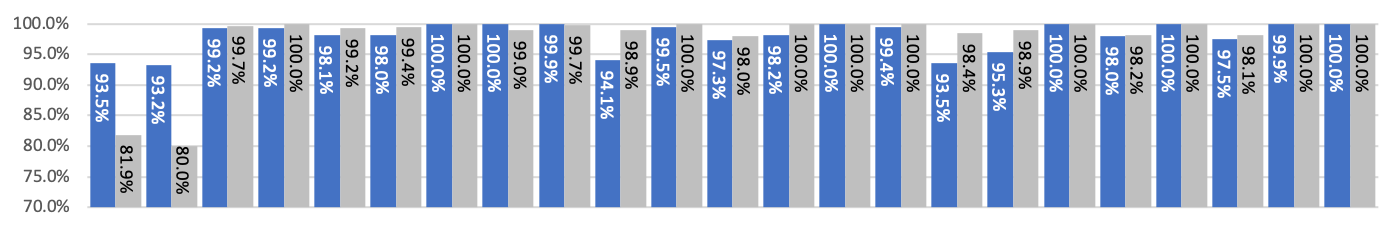
\includegraphics[width=0.92\textwidth]{../results/samnet_cog_orig_canonical_no_labels.png}
  \end{subfigure}%
  \newline
  \begin{subfigure}{\textwidth}
	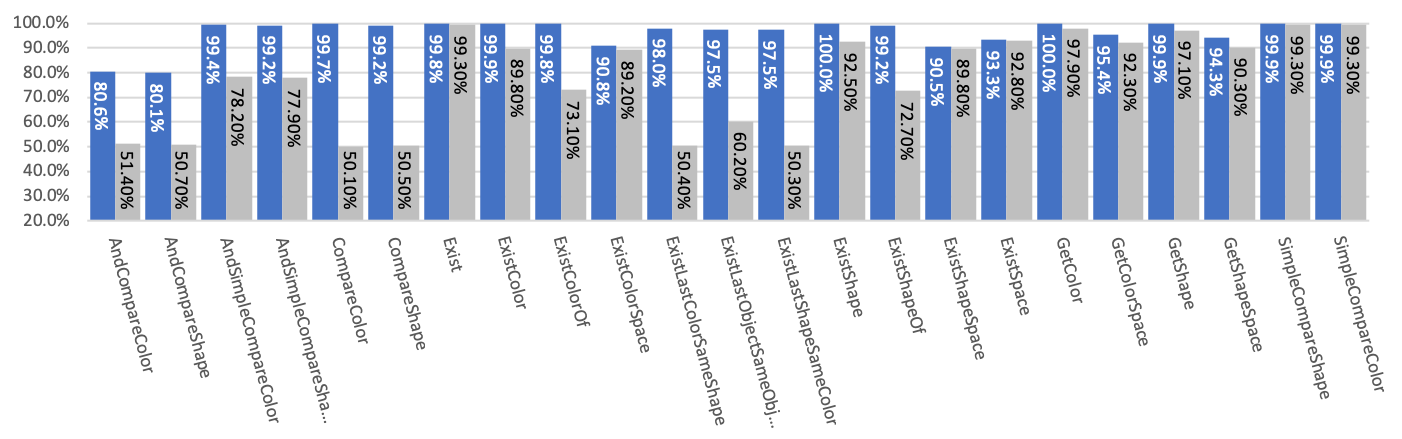
\includegraphics[width=0.93\textwidth]{../results/samnet_cog_orig_hard.png}
  \end{subfigure}%
\caption{Comparison of test set accuracies of SAMNet (blue) with original results achieved by the COG model (gray) on Canonical (top) and Hard (bottom) variants of the COG dataset.}
\label{fig:samnet_cog_detailed}
\end{figure}

\begin{figure}
	\centering
	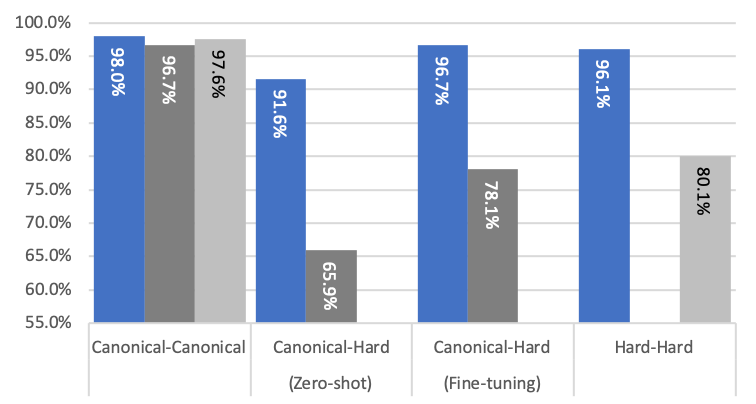
\includegraphics[width=0.75\textwidth]{../results/samnet_cog_overall_transfer.png}
	\caption{Total accuracies of SAMNet (blue) and COG models (light/dark gray) when testing generalization from Canonical to Hard variants of the dataset.}
	\label{fig:samnet_cog_overall_transfer}
\end{figure}

We have implemented and trained our SAMNet model using MI-Prometheus~\cite{kornuta2018accelerating}, a framework based on Pytorch~\cite{paszke2017automatic}. 
In our experiments, we have focused on 22 classification tasks and compared our results with the baseline model, as presented in \cref{fig:samnet_cog_detailed}.
For the Canonical variant (top row), we have achieved similar accuracies for the majority of tasks (with the total average accuracy of 98.0\% in comparison of 97.6\% achieved by the COG model), with significant improvements (around 13 points) for \textit{AndCompare} tasks.
As those tasks focus on compositional questions referring to two objects, we hypothesize that our model achieved better accuracy due to the ability to selectively pick and store the relevant objects from the past frames in the memory.
Despite there being some tasks in which our model reached slightly lower accuracies,
% (between 0.2 and 1.8 points)
when comparing performances on the Hard variant, it improves upon the  COG baseline on all tasks, with improvements varying from 0.5 to more than 30 points.

The goal of the next set of experiments was to test the generalization ability concerning the sequence length and number of distractors.
For that purpose, we have compared the accuracies of both models when trained on the Canonical variant and tested on Hard (\cref{fig:samnet_cog_overall_transfer}).
As the original paper does not include such experiments, we have performed them on our own.  The light gray color indicates the original results, whereas dark gray indicates the accuracies of COG models that we have trained (fine-tuning/testing) using the original code provided by the authors.
For sanity check, in the first column, we report both the best-achieved score and the score reported in the paper when training and testing on Canonical variant, without any fine-tuning.
In a pure \textit{transfer learning} setup (second column), our model shows enormous generalization ability, reaching 91.6\% accuracy on the test set.
We have also tested both models in a setup where the model trained on a Canonical variant underwent additional fine-tuning (for a single epoch) on the Hard variant (third column).
In this case, the SAMNet model also reached much better performance, and, interestingly, achieved better scores from the model trained and tested exclusively on the Hard variant.
In summary, the results clearly indicate that the mechanisms introduced in SAMNet  enable it to learn to operate independently of the total number of frames or number of distractions, and allow it to generalize to longer videos and more complex scenes. One other strength of SAMNet is its interpretability. Observing attention maps (see supplementary material) shows that SAMNet can effectively perform multi-step reasoning over questions and frames as intended. It also accurately classifies temporal contexts as designed. However we notice that the model can sometime discover alternative strategies that were not in the intended design but the answers are still correct. 

%we used the canonical (easy) and hard settings that alter the number of distractors and sequence length.  Since there was no baseline for these tests (train on canonical, test on hard), we ran our own experiments using the COG model provided by the authors.  SAMNet achieves the highest overall scores for all categories of experiments (\cref{fig:samnet_cog_overall_transfer}), especially for the tests run on the hard dataset.  Among the 22 classification tasks, we highlighted the two most difficult tasks that affect the overall score. 
%We argue that the generalization capability of SAMNet is mainly due to the dynamic frame-by-frame processing of the input sequence. 
%The mechanisms introduced in SAMCell learn to operate independently of the total number of frames and allow to generalize to longer video lengths.
%As shown in \cref{fig:samnet_cog_overall_transfer}, when trained on the easy dataset, SAMNet still performs 91.6\% when tested on the hard dataset, whereas COG drops from 97.6\% to 65.9\%   The visualization of the trained SAMNet model (see Appendix) indicates that the model learns the concept of time, helping it to control the flow of information from visual input to the memory.  Therefore, the memory is updated efficiently instead of storing all information across all frames.






	
	
	\newpage
	\bibliographystyle{alpha}
	\bibliography{../cog_bibliography}
	
	\newpage
	\section{Appendix}

\section{VWM model}

\begin{notation}
Treat 1D tensors as column vectors and 2D tensors as matrices, where appropriate.
We use lower case to represent both 1D and 2D tensors but occasionally use upper case
for 2D tensors where matrix operations are involved.

\begin{enumerate}
	\item Let 
	$\Delta^d = \{ (x_0, x_1, \dots, x_d) : x_0 + x_1 + \dots + x_d = 1, x_i \ge 0, i = 0, 1, \dots, d\}$ denote the standard $d$-simplex.	
	
	\item  Let $\circ$ denote concatenation of two tensors with identical shape except possibly
	for their last dimensions $d_1$ and $d_2$, respectively,  
	resulting in a tensor with last dimension of $d_1+d_2$. 
	
	\item Let $\odot$ denote  element-wise product of two tensors of same shape,
	i.e., Hadamard product for vectors/matrices.
	
	\item Let $\otimes$ denote tensor product of two tensors, 
	i.e. Kronecker product for vectors/matrices.
\end{enumerate}
\end{notation}	

\section{Basic layers/modules}

\colorbx{Linear (Affine) Layer}

\begin{description}
	\item[Inputs:] A tensor $x$ with last dimension $n$.
	\item[Parameter:] An affine function $\cG: \Reals^n \to \Reals^m$ with 
	weight and bias parameters.
		
	\item[Output:] A tensor $y$ with last dimension $m$, and remaining dimensions
	same as that of $x$, obtained by applying $\cG$ to each 1D slice of $x$
	along the last dimension.
	\end{description}


\colorbx{Attention Module}

\begin{description}
	\item[Inputs:] 
	\begin{enumerate}
		\item[]
		\item Query: $q \in \Reals^d$
		\item Keys: $K \in \Reals^{N \times d}$	
		\item Values: $V \in \Reals^{N \times d}$. By default $V=K$, unless mentioned explicitly.	
	\end{enumerate}

	\item[Parameter:] Weight $w \in \Reals^d$

	\item[Outputs:] 
	\begin{enumerate}
		\item[]
		\item Content vector: $h =  V^{\T} u \in \Reals^d$
		\item Attention vector:  $w = \softmax(K(w \odot q)) \in \Reals^N$
	\end{enumerate}
\end{description}


\colorbx{Interaction Module}

\begin{description}
	\item[Inputs:] 
	\begin{enumerate}
		\item[]
		\item Base object: $b \in \Reals^d$
		\item Feature objects: $f \in \Reals^{M \times d}$	
	\end{enumerate}
	
	\item[Parameters:] 
	\begin{enumerate}
	\item[]
	\item Base object projection linear layer: $\cG: \Reals^d \to \Reals^d$
	\item Feature objects projection linear layer : $\cK: \Reals^{M \times d} \to \Reals^{M \times d}$
	\item Modifier linear layer:  $\cH: \Reals^{M \times 2d} \to \Reals^{M \times d}$	
\end{enumerate}
		
	\item[Output:] Modified feature objects 
	$f' =  \cH( \cK(f) \odot ( \vone \otimes \cG(b))) \in  \Reals^{M \times d}$
\end{description}

\hrulefill

\section{VWM cell}

The VWM recurrent cell is executed for $T$ reasoning steps for every frame in
the temporal order.  Within a single frame, the cell state at the end of each reasoning step 
$t=1,2, \dots, T$ is denoted by $(c_t, M_t, o_t)$, where: 
\begin{enumerate}
	\item $c_t \in \Reals^d$ is the control state;
	\item $M_t \in  \Reals^{N \times d}$ is the visual working memory with $N$ slots;
	\item $w_t \in  \Reals^N$ is the write head; and
	\item $so_t  \in \Reals^d$ is the summary visual object.
\end{enumerate} 
The initial state is such that both $c_0$ and $so_0$ are initialized
to a fixed value at the start of each frame. However $M_0$ is initialized only once at
the start of the first frame and otherwise taken to be the value of $M_T$ at the
end of the previous frame.

%The number of slots $N$ for the VWM $M_t$ is not fixed because the neural network 
%parameters do not depend on it. It can be variable across the different datasets used
%for training, validation and test as well as within each dataset. This, for example, enables a 
%form of transfer learning where we can train on an easy dataset for one value of $N$
%and study its generalization to a hard dataset using a larger value of $N$.

\colorbx{Question-driven Controller}

The Question-driven Controller plays an important role in the reasoning process.
It drives the attention over the question and produces the new control states. Each new control state defines a new reasoning operation. The inputs of this unit are the past control state, the question encoding and the contextual words (see Question Encoding Unit). It uses the dot product attention between the contextual words
and the combination of the past control states and the question encoding.  This attention layer produces the new control state.

This unit also outputs the temporal class weights that will be used in the Reasoning Unit. It gives access to a temporal information for the current words (last, latest, now, none temporal).

\begin{description}
	\item[Inputs:] 
	\begin{enumerate}
		\item[]
		\item Reasoning step $t = 1,2, \dots, T$
		\item Previous control state: $c_{t-1} \in \Reals^d$	
		\item Contextual words: $cw \in \Reals^{L \times d}$
		\item Question encoding: $q \in \Reals^d$
	\end{enumerate}
	
	\item[Parameters:] 
	\begin{enumerate}
		\item[]
		\item Reasoning step-dependent linear layer: $\cG_t: \Reals^d \to \Reals^d$, depending on $s$
		\item Concatenation linear layer: $\cH: \Reals^{2d} \to \Reals^d$
		\item Attention module $\cA$
		\item Temporal classifier:  $\cK: \Reals^d \to \Delta^3$. A two-layer feedforward
		network with ELU activation in the hidden layer of $d$ units.	
		The classes for the temporal context are labeled ``last'', ``latest'', ``now'', as well as 
		a fourth class label ``none`` indicating no temporal context.
		If $\tau \in \Delta^3$ is the output of the classifier, we denote the components by
		$\tlast$, $\tlatest$, $\tnow$ and $\tnone$.
	\end{enumerate}
	
	\item[Outputs:] 
	\begin{enumerate}
		\item[]
		\item Control state $c_t \in \Reals^d$
		\item Control attention $ca_t \in \Reals^L$
		\item Temporal class weights $\tau_t \in \Reals^4$
    \end{enumerate}
	
	\item[Equations:] 
	\begin{enumerate}
		\item[]
		\item Modulation: $y = \cH\bigl([c_{t-1}, \cG_t(q)]\bigr)$
		\item Control state and attention: $c_t,  ca_t= \cA(y, cw)$
		\item Temporal classification: $\tau_t = \cK(c_t)$
\end{enumerate}
\end{description}


\colorbx{Visual Retrieval Unit}

The visual retrievial unit is responsible to extract visual information from the current image given a control state coming from the Question-driven Controller. It is first projecting the past summary object and the feature maps together using the interaction module.
It is then using the attention module as follow. The query are the control states and the keys and are the feature maps coming from the image encoder. The results of this attention is applied on the modified features maps coming from the interaction module.  
This unit outputs the extracted object and the visual attention.

\begin{description}
	\item[Inputs:] 
	\begin{enumerate}
		\item[]
		\item Control state: $c_t \in \Reals^d$	
		\item Previous summary object: $so_{t-1} \in \Reals^d$
		\item Feature map of current frame: $F \in \Reals^{H \times W \times d}$
	\end{enumerate}
	
	\item[Parameters:] 
	\begin{enumerate}
		\item[]
		\item Interaction module $\cI$
		\item Attention module $\cA$
	\end{enumerate}
	
	\item[Outputs:] 
	\begin{enumerate}
		\item[]
		\item Visual object: $vo_t \in  \Reals^d$
		\item Visual attention: $va_t  \in \Reals^{H \times W \times d}$
	\end{enumerate}

	\item[Equations:]
	\begin{enumerate}
		\item[]
		\item Modified feature map: $\hat{F} = \cI(so_{t-1}, F)$
		\item Visual object and attention: $vo_t, va_t = \cA(y, \hat{F}, M_{t-1})$
	\end{enumerate}
\end{description}

\begin{note}
	Appropriate flatten/unflatten operations are performed to match the signature 
	of the modules.
\end{note}


\colorbx{Memory Retrieval Unit}

The role of the memory retrieval unit is to read and extract object from memory).
As the Visual Retrieval Unit, it uses the combination of the two following submodules. The interaction module blends together the extracted object and the content of the memory. The attention module then extract the corresponding object in memory if present. This unit outputs the extracted object and its corresponding location, we call it the "read head".

\begin{description}
	\item[Inputs:] 
	\begin{enumerate}
		\item[]
		\item Control state: $c_t \in \Reals^d$	
		\item Previous summary object: $so_{t-1} \in  \Reals^d$
		\item Previous VWM $M_{t-1} \in \Reals^{N \times d}$
	\end{enumerate}
	
	\item[Parameters:] 
	\begin{enumerate}
		\item[]
		\item Interaction module $\cI$
		\item Attention module $\cA$
	\end{enumerate}
	
	\item[Outputs:] 
	\begin{enumerate}
		\item[]
		\item Memory object: $mo_t \in \Reals^d$
		\item Read head: $\rhead_t \in \Reals^N$
	\end{enumerate}

	\item[Equations:]
	\begin{enumerate}
		\item[]
		\item Modified VWM: $\hat{M}_t = \cI(so_{t-1}, M_{t-1})$
		\item Memory object and attention: $mo_t, \rhead_t = \cA(y, \hat{M}_t, M_{t-1})$
	\end{enumerate}
\end{description}


\colorbx{Reasoning Unit}

%control_state, visual_object, memory_object, temporal_class_weights

\begin{description}
	\item[Inputs:] 
	\begin{enumerate}
		\item[]
		\item Control state: $c_t \in \Reals^d$
		\item Visual object: $vo_t \in \Reals^d$
		\item Memory object: $mo_t \in \Reals^d$
		\item Temporal class weights $\tau \in \Delta^3$
	\end{enumerate}
	
	\item[Parameters:] Validator modules $\cG, \cK: \Reals^{2d} \to \Reals$.
	Both $\cG, \cK$ are two-layer networks of $2d$ hidden units,
	using ELU activation in the hidden layer, and sigmoid in the output layer.
	
	\item[Output:] Predicate gates for the current reasoning step
	\begin{enumerate}
    	\item Object match predicate gates (i) image: $\imatch_t \in [0,1]$ and 
    	(ii) memory: $\mmatch_t \in [0,1]$.
		
		\item Memory update predicate gates (i) add: $\doadd_t \in [0,1]$ and
		(ii) replace: $\doreplace_t \in [0,1]$
    \end{enumerate}

	\item[Equations:]
	\begin{enumerate}
		\item[]
		\item $\imatch_t \in [0,1]$:
		It's true if there is a valid visual object. This assumes that
		the current reasoning step refers to either ```now''  or ``latest''.
		
		\item$\mmatch_t \in [0,1]$:
		It's true if there is a valid memory object. This assumes that
		the current reasoning step refers to either ``last'',  or alternatively ``latest'' 
		but there is no matching visual object.
		
		\item $\doadd_t$:
		
		
		\item $\doreplace_t$: 
\end{enumerate}
\end{description}


\colorbx{Memory Update Unit}

This unit is meant to update the content of the memory. 

Three actions can happen:

\begin{itemize}
	\item There is no object to be added to memory, the memory remains unchanged
	\item There is one object that needs to be added to memory, but a similar object is already in memory at a given location. The new object will replace the old object at this location
	
	\item There is one object that needs to be added to memory, and  it is a new object. It is added at the write head location.
\end{itemize}


This module also updates the position of the write head. If a new object as been added to the current write head position, the right head shifts right to a new empty slot. If the object has been replaced, the write head doesn't move.
% visual_object, visual_working_memory, read_head, write_head, do_replace, do_add_new

\begin{description}
	\item[Inputs:] 
	\begin{enumerate}
		\item[]
		\item Visual object: $vo_t \in \Reals^d$
		\item Memory object: $mo_t \in \Reals^d$
		\item Memory update predicate gates:  $\doadd_t, \doreplace_t \in [0,1]$
		\item Read head: $\rhead_t \in \Reals^N$
		\item Previous VWM $M_{t-1} \in \Reals^{N \times d}$
		\item Previous write head: $\whead_{t-1} \in \Reals^N$
	\end{enumerate}

	\item[Outputs:] 
	\begin{enumerate}
		\item[]
		\item VWM $M_t \in \Reals^{N \times d}$
		\item Read head: $\rhead_t \in \Reals^N$
		\item Write head: $\whead_t \in \Reals^N$
	\end{enumerate}

\end{description}



\colorbx{Summary Object Update Unit}

The  Summary Unit is the last unit of the SAMCell. It is responsible to output the new summary object. It first picks which object is relevant between the object extracted from memory and the visual object extracted from the image. Once the relevant object is picked, it is combined with the former summary object through a linear layer to become the new summary object. It is the final step of the SAMCell reasoning cycle. 

The image encoder, question encoder and output unit are described in the appendix.

\begin{description}
	\item[Inputs:] 
	\begin{enumerate}
		\item[]
		\item Previous summary object: $so_{t-1} \in \Reals^d$
		\item Visual object: $vo_t \in \Reals^d$
		\item Memory object: $mo_t \in \Reals^d$
		\item Object predicate gates: $\imatch_t, \mmatch_t \in [0,1]$
	\end{enumerate}
	
	\item[Parameters:] Concatenation linear layer $\cH$ 
	
	\item[Output:] 
     New summary object:
	             $so_t = \cH\bigl([so_{t-1}, (\imatch_t * vo_t + \mmatch_t * mo_t)]\bigr) \in \Reals^d$ 
	
\end{description}


\noindent\makebox[\linewidth]{\rule{\paperwidth}{1pt}}



\begin{figure}
	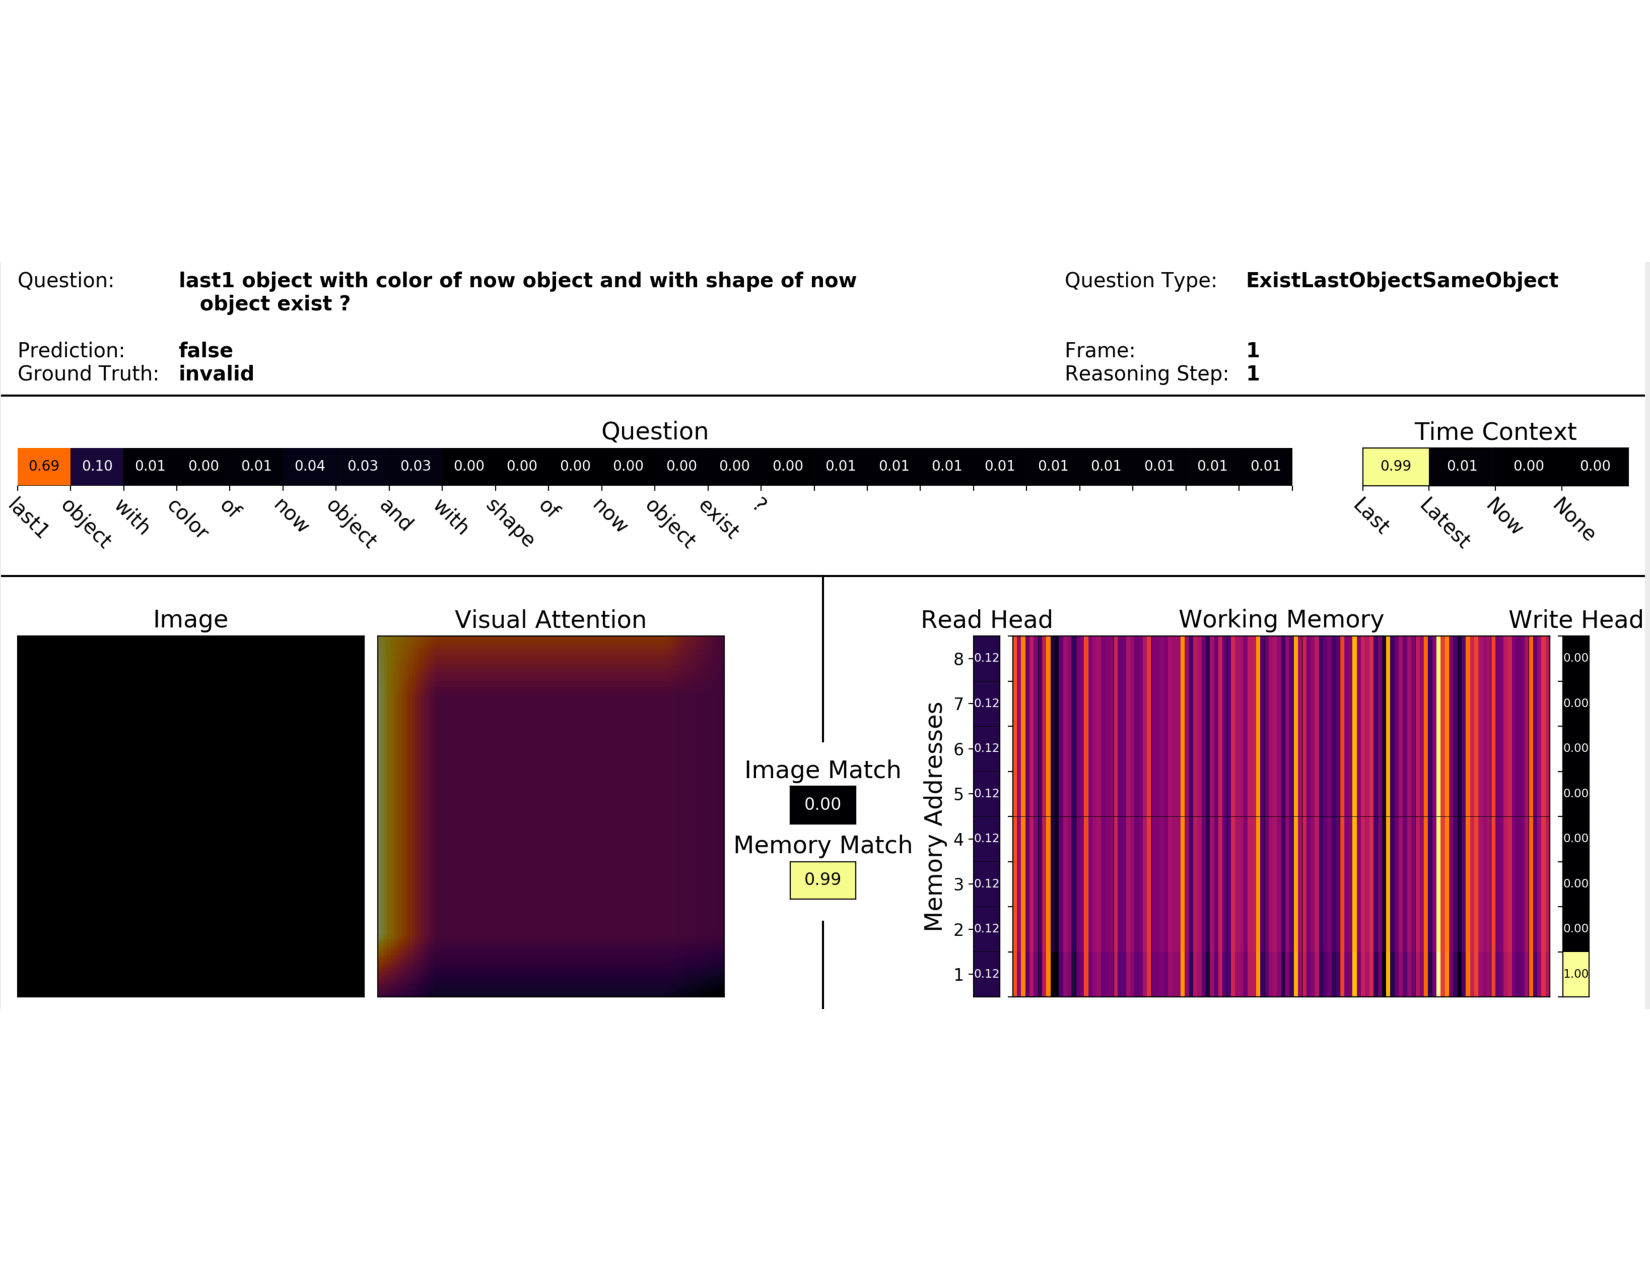
\includegraphics[width=\textwidth]{img/model2}
	\label{fig:model}
\end{figure}	

\begin{figure}
	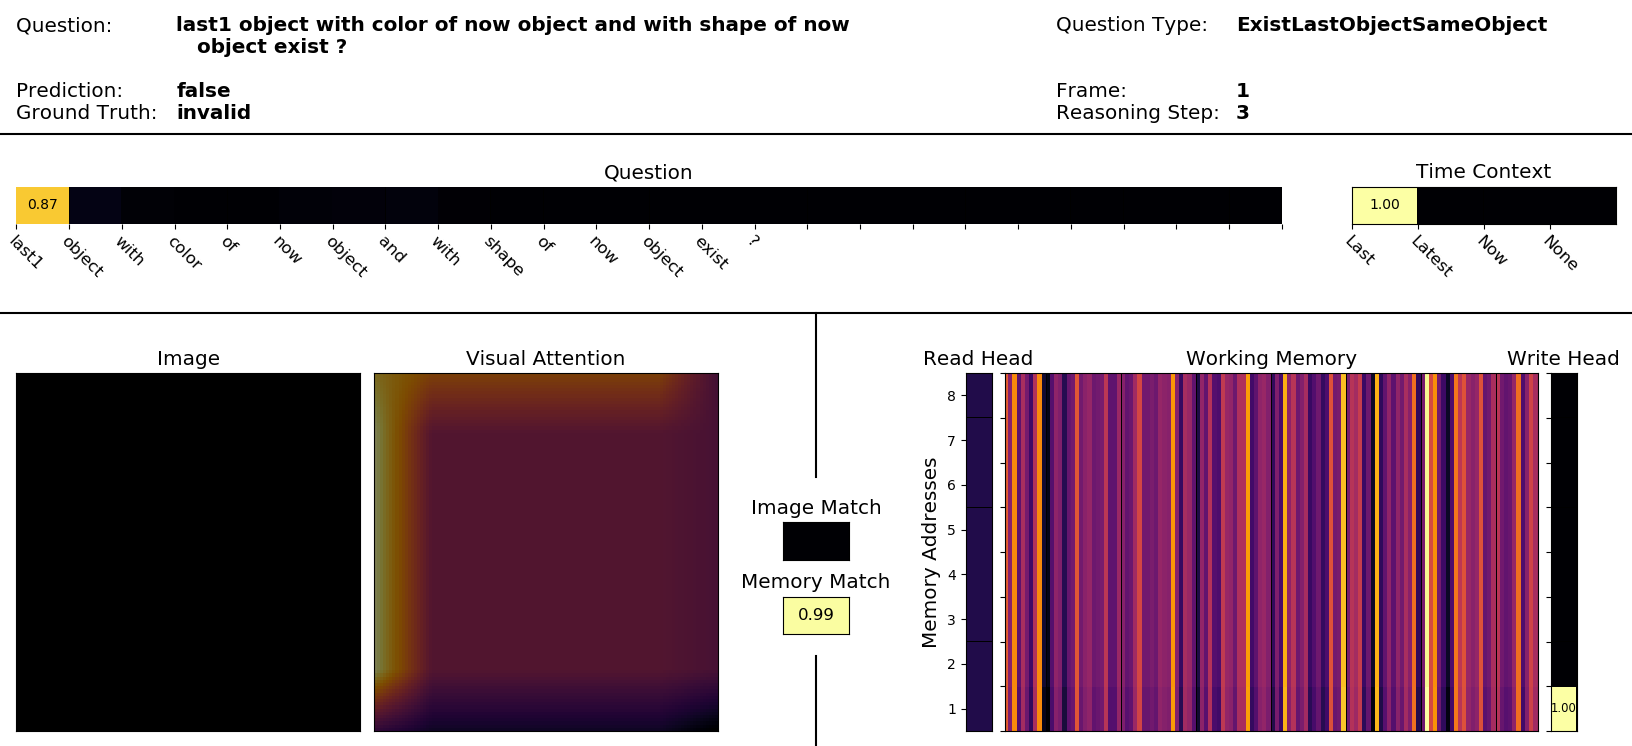
\includegraphics[width=\textwidth]{img/image}
	\label{fig:model}
\end{figure}	

\colorbx{Image Encoder}

\colorbx{Question Encoder}

\colorbx{Output Unit}

\section{Training and Implementation Details}

SAMNet is implemented on IBM's Mi-Prometheus~\cite{kornuta2018accelerating} framework based on Pytorch. 
We trained all our models using NVIDIA’s GeForce GTX TITAN X GPUs. SAMNet was trained using 8 reasoning steps and a hidden state size of 128. The external memory has 128-bit slots for all experiments. We trained our model until convergence but we also have set a training time limit of 80 hours.


\section{Results}


\begin{table}[t]
	\tiny
	
	\caption{COG test set accuracies for  SAMNet \& COG models. For the COG section, the results marked as 'paper' comes from the original COG paper ~\cite{yang2018dataset}, whereas the results marked as 'ours' come from our own experiments using the following implementation: https://github.com/google/cog }
	
	\resizebox{\textwidth}{!}{
	\centering
	\begin{tabular}{ccccccccccc}
		\toprule
		Model & & SAMNet & && && COG&& \\
		\cmidrule{2-5} \cmidrule{7-11} 
		&&&&& & paper & ours & ours & paper&\\
		\cmidrule{7-9} \cmidrule{10-11}
		Trained on       & canonical & canonical & canonical & hard &           &  canonical  & canonical  & canonical & hard \\ 
		Fine tuned on  & - & - & hard  & - &           & -   & - & hard & - \\ 
		Tested on        & canonical & hard & hard & hard &            &canonical  & hard & hard & hard  \\ 
		\midrule
		
		Overall accuracy & 98.0 & 91.6 & 96.5  & running &           & 97.6  & 65.9 & running& 80.1 \\ 
		
		\midrule 
		
		
		AndCompareColor	&	93.5		&	82.7	&	89.2	&&		&81.9	&57.1&&	51.4
		\\ 
		AndCompareShape	&	93.2 		&	83.7	&	89.7	&&	&	80.0	&53.1	&&50.7\\ 
		AndSimpleCompareColor	&	99.2	&		85.3	&	97.6	&	&	&99.7&	53.4&&	78.2\\ 
		AndSimpleCompareShape	&	99.2&			85.8	&	97.6	&&	&	100.0	&56.7&&	77.9\\ 
		CompareColor	&	98.1		&	89.3	&	95.9	&&		&99.2&	56.1&&	50.1\\ 
		CompareShape	&	98.0	&		89.7	&	95.9	&&	&99.4	&66.8	&&50.5
		\\ 
		Exist	&	100.0	&		99.7	&	99.8		&&	&	100.0&	63.5&&	99.3\\ 
		ExistColor	&	100.0		&	99.6	&	99.9	&&	&	99.0&	70.9&&	89.8\\ 
		ExistColorOf	&	99.9	&		95.5	&	99.7		& & &	99.7&	51.5&&	73.1\\ 
		ExistColorSpace	&94.1		&	88.8	&	91.0	&& &	98.9	&72.8	&&89.2\\ 
		ExistLastColorSameShape	&	99.5		&	99.4	&99.4	&&		&100.0	&65.0&&	50.4
		\\ 
		ExistLastObjectSameObject	&	97.3	&		97.5	&	97.7	&&	&	98.0&	77.5	&&60.2\\ 
		ExistLastShapeSameColor	&	98.2		&	98.5&	98.8	&&	&	100.0&	87.8&&	50.3\\ 
		ExistShape	&	100.0	&	99.5	&	100.0	&&&	100.0&	77.1	&&92.5\\ 
		ExistShapeOf	&	99.4		&	95.9	&	99.2	&&&100.0	&52.7&&89.8\\ 
		ExistSpace	&	95.3	&	89.7	&	93.2	&&		&	98.9	&71.1	&&92.8\\ 
		GetColor	&	100.0		&	95.8&	99.9	&& &	100.0&	71.4&&	97.9\\ 
		GetColorSpace	&	98.0		&	90.0	&	95.0&	& &	98.2	&71.8&&	92.3\\ 
		GetShape	&	100.0		&	97.3&	99.9&	&	&	100.0  &83.5&&	97.1
		\\ 
		GetShapeSpace	&	97.5	&	89.4	&	93.9	&&&	98.1  &78.7	&&	90.3\\ 
		SimpleCompareShape	&	99.9		&	91.4	&	99.7	&	&&	100.0 & 67.7&&	99.3\\ 
		SimpleCompareColor	&	100.0 		&	91.6  &	99.80&	&	&	100.0&	64.2&&	99.3	  \\ 
		
		
		
		
		
		
		
		\bottomrule
	\end{tabular}
}

	\label{results}
\end{table}



	
\end{document}
